% Packages
\documentclass{article}
\usepackage{graphicx} % Required for inserting images
\graphicspath{{../figures/}{figures/}{./}} % repo layout: main.tex in paper/, figures in ../figures/

% Edit document margins
\usepackage[
    top=1in,
    bottom=1in,
    left=1.1in,
    right=1.3in
]{geometry}

\usepackage{float}
\usepackage{listings}
\usepackage{xcolor}
\usepackage{microtype}
\usepackage{caption}
\usepackage{parskip}
\usepackage[hyphens]{url}
\usepackage{hyperref}
\usepackage[most]{tcolorbox}

\documentclass{article}
\usepackage[margin=1in]{geometry}
\usepackage{fancyhdr}
\usepackage{booktabs}
\usepackage{tabularx}
\usepackage{threeparttable}
\pagestyle{empty}


%Begin Document
\begin{document}

% Title
\begin{titlepage}
\thispagestyle{empty}
\vspace*{2.5cm}

{\fontsize{30}{34}\selectfont\bfseries
Buying World Cup Wins
\par}

\vspace{0.25cm}

{\fontsize{20}{24}\selectfont\bfseries
and Historical Determinism
\par}

\vspace{0.6cm}

\rule{0.65\textwidth}{0.7pt}

\vspace{1cm}

{\Large
STATS 418: Final Project
}

\vfill

{\large
Jeremy Shiu \hspace{1cm} Rachel Nguyen
}

\vspace{0.4cm}

{\large
University of California, Los Angeles
}

\vspace{0.3cm}

{\large
July 2026
}

\end{titlepage}

% Footer
\pagestyle{fancy}
\fancyhf{}                  % Clear all headers and footers
\fancyfoot[R]{\thepage}             % Bottom right
\renewcommand{\headrulewidth}{0pt} % Remove header line
\renewcommand{\footrulewidth}{0pt} % Remove footer line

% Table of Contents
\clearpage
\tableofcontents
\clearpage



% Executive Summary
\begin{tcolorbox}[
    colback=gray!8,
    colframe=gray!8,
    sharp corners,
    boxrule=0pt
]
\textbf{\large Executive Summary}

\vspace{1.0em}

This study examines which team characteristics are most strongly associated with advancing beyond the FIFA World Cup group stage. Using  a logistic regression model, we estimate how prior tournament experience, host status, squad composition, and contextual factors influence the probability of advancement.
\vspace{0.8em}

Three findings emerge. First, hosting the tournament produces the largest observed effect, raising advancement odds roughly eightfold ($p \approx .002$). Second, tournament experience provides a measurable, compounding advantage: each additional prior World Cup appearance increases the odds of advancing by roughly 22\% ($p < .001$). Third, even after accounting for the other factors, meaningful regional differences remain, with UEFA and CONMEBOL teams consistently outperforming AFC, CAF, and CONCACAF.
\vspace{0.8em}

The resulting model correctly classifies approximately 71\% of historical group-stage campaigns and achieves an AUC of 0.79 in sample, demonstrating meaningful predictive power while remaining easy to interpret. The model quantifies which characteristics historically matter most, providing an evidence-based framework for evaluating competitive advantage before a tournament begins. The signal holds up out of sample: trained on tournaments before 2010 and tested on 2010--2022, the model retains 65\% accuracy and an AUC of 0.69, and it achieves a forward-test AUC of 0.757 on the completed 2026 field. 

\end{tcolorbox}




\vspace{2.8em}

% Background
\section{Business Context}

\vspace{1.2em}

\textbf{\large Why World Cup Group Stage Advancement Matters} 

The FIFA World Cup is one of the most difficult sporting events to forecast, owing to its infrequent occurrence, limited number of matches, and high competitive parity. Yet the stakes make accurate forecasts valuable: the 2022 tournament generated roughly \$7.6B in revenue, drew about 6.6M fans across 102 matches, and engaged an estimated 5B viewers across television and digital platforms. Sports organizations, broadcasters, analysts, and betting markets all have a stake in evaluating tournament performance and strategic decision-making ahead of kickoff.

The FIFA World Cup begins with a \emph{group stage}, in which teams are divided into groups and compete in a round-robin format, with the top finishers from each group advancing to the knockout stage and the remainder eliminated. In the expanded 2026 format, 48 teams compete and roughly two-thirds advance --- 32 teams move on and 16 are eliminated (Figure~\ref{fig:progression}).

As a result, advancing beyond the group stage represents the tournament's first major competitive milestone and may set a team up on a more favorable path through the knockout rounds.

\vspace{1.2em}

\textbf{\large Study Objective} 

This study identifies the team characteristics most associated with advancing beyond the FIFA World Cup Group Stage. Using historical World Cup data, we develop a logistic regression model that estimates how factors such as tournament experience, squad composition, and contextual variables influence the probability of advancement.

Beyond generating predictions, the model provides estimates that quantify the relative importance of each predictor, offering practical information for forecasting tournament outcomes and evaluating competitive advantage.




% Data and Methodology
\section{Data \& Methodology}
The analysis uses an open-source relational World Cup database (datahub.io). It contains 38 linked tables of tournaments, teams, squads, players, matches, bookings, host nations, and managers dating back to 1930.

Datasets were constructed in SQL (using \texttt{sqldf} in R) by joining the tournament, team, player, and manager tables into a single data frame. The unit of analysis is a single team's group-stage campaign in a single men's FIFA World Cup. After restricting to men's tournaments from 1970 onward, the modeling table contains 366 team-campaigns. The resulting predictor variables are summarized in Table~\ref{tab:predictors}; the full SQL construction query is available in the Appendix~\ref{sec:sql}.  
\vspace{0.3 em}

\begin{table}[H]
\centering
\caption{Predictor Variables}
\label{tab:predictors}


\begin{threeparttable}
\renewcommand{\arraystretch}{1.25}
\begin{tabularx}{\textwidth}{@{} l X c @{}}
\toprule
\textbf{Variable} & \textbf{Description} & \textbf{Type} \\
\midrule
Team Experience & Previous FIFA World Cup appearances. & Numeric \\

Squad Composition & Average squad age, squad size, and positional composition. Average age is calculated as tournament year minus birth year.\tnote{a} & Numeric \\

Squad World Cup Experience & Average prior World Cup appearances per player. & Numeric \\

% Cards (Discipline) & Total number of yellow and red cards received by the team during the group stage. & Numeric \\

Host Nation Flag & Indicator variable equal to 1 if the team is playing in its home country and 0 otherwise. & Binary \\

Foreign Manager Flag & Indicator variable equal to 1 if the team's head coach is from a different country than the team and 0 otherwise. & Binary \\

\bottomrule
\end{tabularx}
\begin{tablenotes}
\footnotesize
\item[a] Players with missing birth dates (78 total) are excluded from the age calculation.
\end{tablenotes}
\end{threeparttable}
\end{table}

\vspace{1.2em}
\textbf{\large Data Cleaning}

As part of data cleaning, we made several decisions to ensure the analysis was scoped correctly and the model's estimates were stable. This included restricting the dataset to comparable tournaments and removing redundant predictor variables:


\textbf{Tournaments after 1970}: Penalty card records before 1970 are unavailable, so those tournaments were excluded to avoid treating missing values as clean play. In addition, the tournament format changed after 1970, so this restriction also ensures a consistent three-match group stage for each team, although qualification rules and tie-break procedures have still changed over time within the scope of our final data.

\textbf {Men's Tournaments}: The dataset includes both men's and women's World Cup tournaments. We restricted the analysis to men's tournaments because the two are separate competitions with different histories, tournament counts, and formats, and mixing them would undermine the comparability of the results. We utilized some regular expressions here to clean up the labels and make sure we kept the correct rows.

\textbf{Missing Values}: Missing card, host, or manager values were coalesced
to 0 where a legitimate zero (e.g. not a host) was the
correct interpretation.

\textbf{Collinearity and redundancy.} We excluded variables that directly reflected tournament outcomes (e.g., wins, draws, losses, goals for, goals against, goal difference, and points) and removed redundant correlated predictors to ensure the logistic regression estimated the independent effects of pre-tournament characteristics with stable, interpretable coefficients.

\vspace{2.8em}
\textbf{\large Data Processing}

The primary outcome for the logistic model is a binary \texttt{advanced} flag indicating whether a team finished high enough in its group to reach the knockout stage. For the exploratory point-based models we also constructed \texttt{points\_std} (0--9), a standardized group-stage point total computed with a single 3-1-0 scoring rule (3 for a Win, 1 for a Draw, 0 for a Loss) applied uniformly across eras in place of the raw \texttt{points} column, whose scoring rule changed in 1994.


\noindent Engineered features included \texttt{avg\_prior\_wc} (Squad World Cup Experience; mean prior World Cup appearances per squad member), \texttt{avg\_age} and \texttt{forward\_share}/\texttt{defender\_share} (Squad Composition), \texttt{prior\_tournaments} (Team Experience), \texttt{is\_host} (Host Nation Flag), and \texttt{foreign\_manager}. Confederation (\texttt{conf}) enters as a categorical predictor with UEFA as the baseline.


\vspace{1.8em}

\section {Exploratory Data Analysis}

Before any model was fit, three predictors already showed distinct, consistent relationships with group-stage success.

\textbf{Host status.} Host nations advance far more often than visitors: 87\% of hosts advance, compared with 52\% of non-hosts, and hosts also accumulate more standardized group-stage points on average (Figure~\ref{fig:eda-host}). The gap is consistent with a meaningful home-field advantage.

\textbf{Tournament experience.} Experienced teams tend to advance more often than first-time participants. Advancement rates rise from about 28\% for debut teams to about 76\% for teams with six or more prior appearances --- roughly a threefold difference --- suggesting experience partly proxies for durable team quality (Figure~\ref{fig:eda-exp}).

\textbf{Regional affiliation.} South American (CONMEBOL) and European (UEFA) teams outperform the other confederations, averaging 5.4 and 4.7 standardized group-stage points respectively, while AFC, CAF, and CONCACAF sides cluster well below them (Figure~\ref{fig:eda-conf}). A count-scaled view of goals for versus goals against (Figure~\ref{fig:eda-goals}) shows the offensive/defensive balance underlying these outcomes.

These differences are descriptive; the logistic regression that follows tests whether each pattern persists after accounting for experience, host status, region, and squad characteristics simultaneously. We note the structure of the outcome: \texttt{points\_std} spans 0--9 but a value of 8 is structurally impossible over three matches, and the advancement base rate is roughly 54\%.


\vspace{1.8em}

\section{Modeling}

There were 3 main models that we considered for this analysis: Poisson regression, Ordinal regression, and Logistic regression.

    \textbf{Poisson Regression} was considered for this analysis over a standard linear model due to the bounded nature of our predicted variable. However, the group stage points are not evenly spaced out (it's not possible to get 8 points), and the right side of the distribution does not go to infinity. This meant that we ultimately did not go with this model.
    \vspace{0.8em}
    
    \textbf{Ordinal Regression} was the next choice that made the most sense, as it provided us with an ordered scale representation for the various "degrees" of group stage success without relying on true numeric distance for the calculations. Ultimately, however, we chose to go with the Logistic regression model to ease model interpretation and give us a slightly more meaningful result (qualified or not qualified) to the average viewer.
    \vspace{0.8em}

    
\textbf{Logistic Regression} was selected as the final model because it aligned with the study objective while remaining highly interpretable. The model predicts a binary outcome—whether a team advanced from the group stage—allowing estimated effects to be interpreted through odds ratios that quantify changes in the odds of advancement.

Conceptually, the model estimates advancement using the following team characteristics:

\[
\textbf{Advanced}
=
\text{Prior Tournaments}
+
\text{Host Nation}
+
\text{Confederation}
+
\text{Other Covariates}
\]

Formally, the logistic regression models the log-odds of advancement as

\[
\log\left(
\frac{P(\text{Advanced}=1)}
{1-P(\text{Advanced}=1)}
\right)
=
\beta_0
+
\beta_1(\text{Prior Tournaments})
+
\beta_2(\text{Host Nation})
+
\beta_3(\text{Confederation})
+
\cdots
+
\beta_kX_k.
\]

Although this approach does not distinguish between teams that narrowly advance and those that dominate the group stage, advancement itself is the primary outcome of interest. This tradeoff substantially improves model interpretability while remaining aligned with the study objective.

Logistic regression assumes independent observations, a linear relationship between continuous predictors and the log-odds of the response, limited multicollinearity, and an adequate sample size. The modeling approach and study design were selected to reasonably satisfy these assumptions.

\vspace {1.8em}
\section{Key Findings}

Three factors reliably and meaningfully predict group stage advancement, holding all other variables constant. (Figure~\ref{fig:or}):

\begin{enumerate}

\item \textbf{Hosting provides the largest measurable advantage.} 
Host nations are approximately eight times more likely to advance than comparable non-hosts, highlighting the substantial impact of home support and familiarity.

\item \textbf{Tournament experience predicts success.}
Each prior World Cup appearance increases a team's odds of advancing by approximately 22\%, suggesting that institutional experience compounds over successive tournaments.

\item \textbf{Regional differences remain after controlling for team quality.} 
Relative to UEFA (Europe) teams, AFC (Asia), CAF (Africa), and CONCACAF (North, Central America, and the Caribbean) teams have significantly lower odds of advancing. CONMEBOL (South America) teams perform comparably to UEFA teams.

\end{enumerate}

\vspace{0.8em}

% \begin{figure}[H]
%     \centering
%     \includegraphics[width=0.75\linewidth]{Screenshot 2026-07-29 at 11.36.54 AM.png}
%     \caption{Estimated odds ratios for advancing beyond the Group Stage}
%     \label{fig:placeholder}
% \end{figure}

\vspace{1.2em}

\textbf{\large What Does Not Move the Needle}

Squad age, the mix of forwards versus defenders, and whether a team's manager
is foreign-born showed no statistically detectable effect on advancement odds
once experience, host status, and region are accounted for. This is a useful
negative result: narratives that pin advancement on squad youth or hiring a
foreign coach are not supported by the historical data.

\vspace{1.2em}
\clearpage

\textbf{\large How Much Better Is This Than Guessing}

Historically, 50\% of group-stage campaigns end in advancement, so a naive
model that always guesses "advances" is already right just over half the
time. Beating that baseline on the data used to fit the model is expected, so we
judge the model on tournaments it never saw.

We split the campaigns chronologically rather than at random: the model is fit
on the ten tournaments from \textbf{1970 through 2006} (239 campaigns) and
scored on the four most recent, \textbf{2010 through 2022} (127 campaigns).
A chronological split is the best method for a forecasting model because it
mirrors the overall goal of the model (to predict the future), and it guarantees that no information from
the test years leaks into the fit. 

On that held-out era the model classifies \textbf{65\%} of campaigns correctly
against a \textbf{50\%} naive baseline in those years, a 15-point lift, and
ranks teams by advancement probability with an \textbf{AUC of 0.69}, where
0.50 is a coin flip and 1.00 is perfect separation (Figure~\ref{fig:roc}). Overall, this demonstrates a model that significantly improves over a blind guess, but it clearly has some confounders that further explain results. 


\vspace{1.2em}

\textbf{\large Validating on the 2026 World Cup Tournament}

The 2026 tournament expanded from 32 to 48 teams and changed the qualification rule (top two plus a set of best third-place finishers). We scored the completed 2026 field as a genuine forward test, dropping New Zealand (the lone OFC team, absent from the training data) to leave 47 teams. The model orders the field well, achieving a forward-test AUC of 0.757, where many favorites to advance such as England, Brazil, Argentina, and Spain sit at the top of the odds to advance and low-experience AFC and CAF teams sit at the bottom, right in line with the 2010-split result (Figure~\ref{fig:rank2026}).

Headline accuracy, however, tells a more cautious story. At a 0.5 threshold the model reaches 0.681 accuracy, correctly calling 19 of the teams that advanced and 13 of those eliminated, against 2 false positives and 13 false negatives (Figure~\ref{fig:cm2026}). Because the expanded 48-team format advances roughly two-thirds of teams, that accuracy exactly equals the no-information base rate: even a trivial "everyone advances" rule would score 0.681. The 13 missed teams are genuine Cinderellas buried in the low-probability tail, upsets that a pre-tournament experience-and-region model structurally cannot foresee. AUC, not accuracy, is the honest read for 2026, and any probability estimate for a 2026 team should be treated as provisional given the format change.


\vspace{1.8em}
\section{Business Implications}

The findings demonstrate that \textbf{long-term organizational factors are stronger predictors of World Cup success than many commonly discussed roster characteristics}. Historical tournament experience and host status consistently improve advancement odds, while variables such as average squad age, positional composition, and hiring a foreign manager show no statistically significant effect after controlling for other factors.

For \textbf{national football associations}, these results suggest that investments in sustained international tournament participation and player-development pipelines may yield greater long-term returns than short-term roster adjustments such as changing squad age or manager nationality.

For \textbf{analysts and broadcasters}, tournament experience, host status, and confederation provide a more evidence-based foundation for pre-tournament forecasts than narrative-driven predictions.

For \textbf{forecasting and betting markets}, the same three drivers offer a quantified, defensible baseline for pricing advancement probability ahead of a tournament.

Although the model was developed on historical tournaments, it also provides a baseline for evaluating future competitions. Because the 2026 FIFA World Cup introduced an expanded format that changes advancement dynamics, the estimated relationships should be interpreted as directional rather than definitive, and future tournaments should be re-evaluated as additional data become available. The model maintained reasonable discrimination on the 2026 field (AUC $\approx$ 0.76) despite the format change.
\clearpage

\appendix
\section{Figures}

% Each figure is placed alone on its own page and vertically centered via the
% surrounding \vspace*{\fill} glue; \clearpage flushes the page after each.
\vspace*{\fill}
\begin{figure}[H]
    \centering
    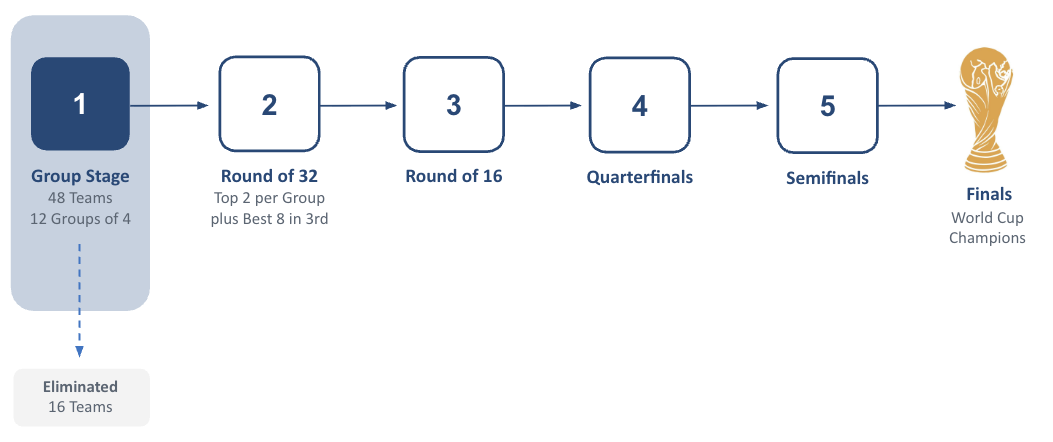
\includegraphics[width=0.7\linewidth]{groupstage}
    \caption{FIFA World Cup tournament progression. In the 2026 format, 48 teams compete, 32 advance beyond the group stage, and 16 are eliminated.}
    \label{fig:progression}
\end{figure}
\vspace*{\fill}
\clearpage

\vspace*{\fill}
\begin{figure}[H]
    \centering
    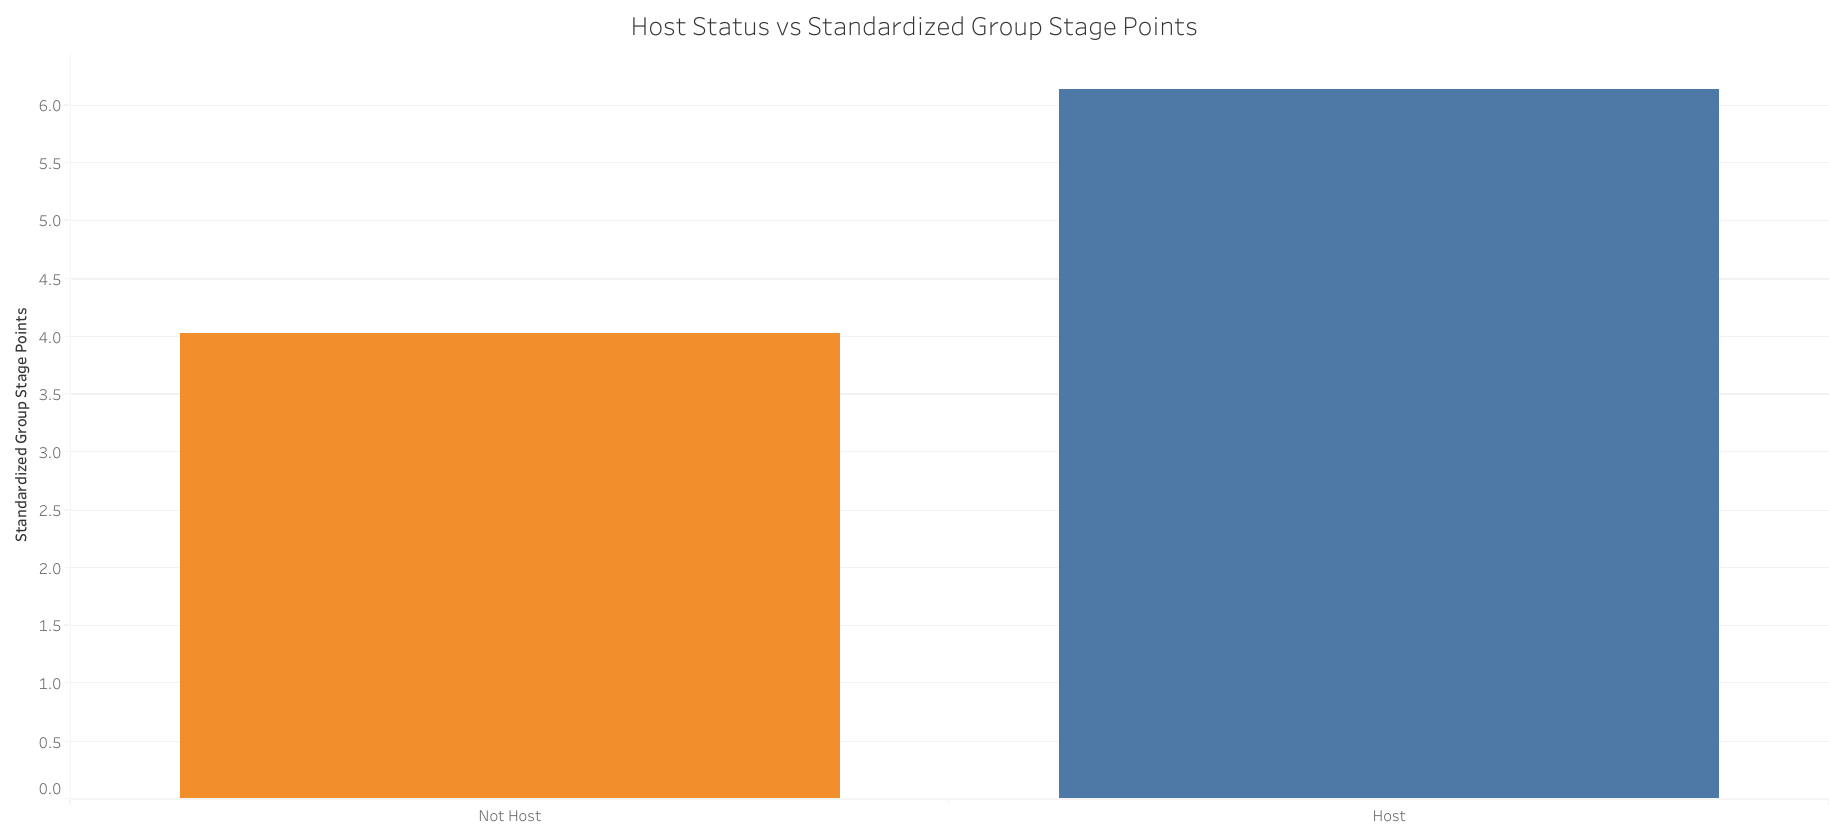
\includegraphics[width=0.75\linewidth]{Host Status vs Standardized Group Stage Points}
    \caption{EDA: host nations accumulate more standardized group-stage points than non-hosts (87\% of hosts advance vs.\ 52\% of non-hosts).}
    \label{fig:eda-host}
\end{figure}
\vspace*{\fill}
\clearpage

\vspace*{\fill}
\begin{figure}[H]
    \centering
    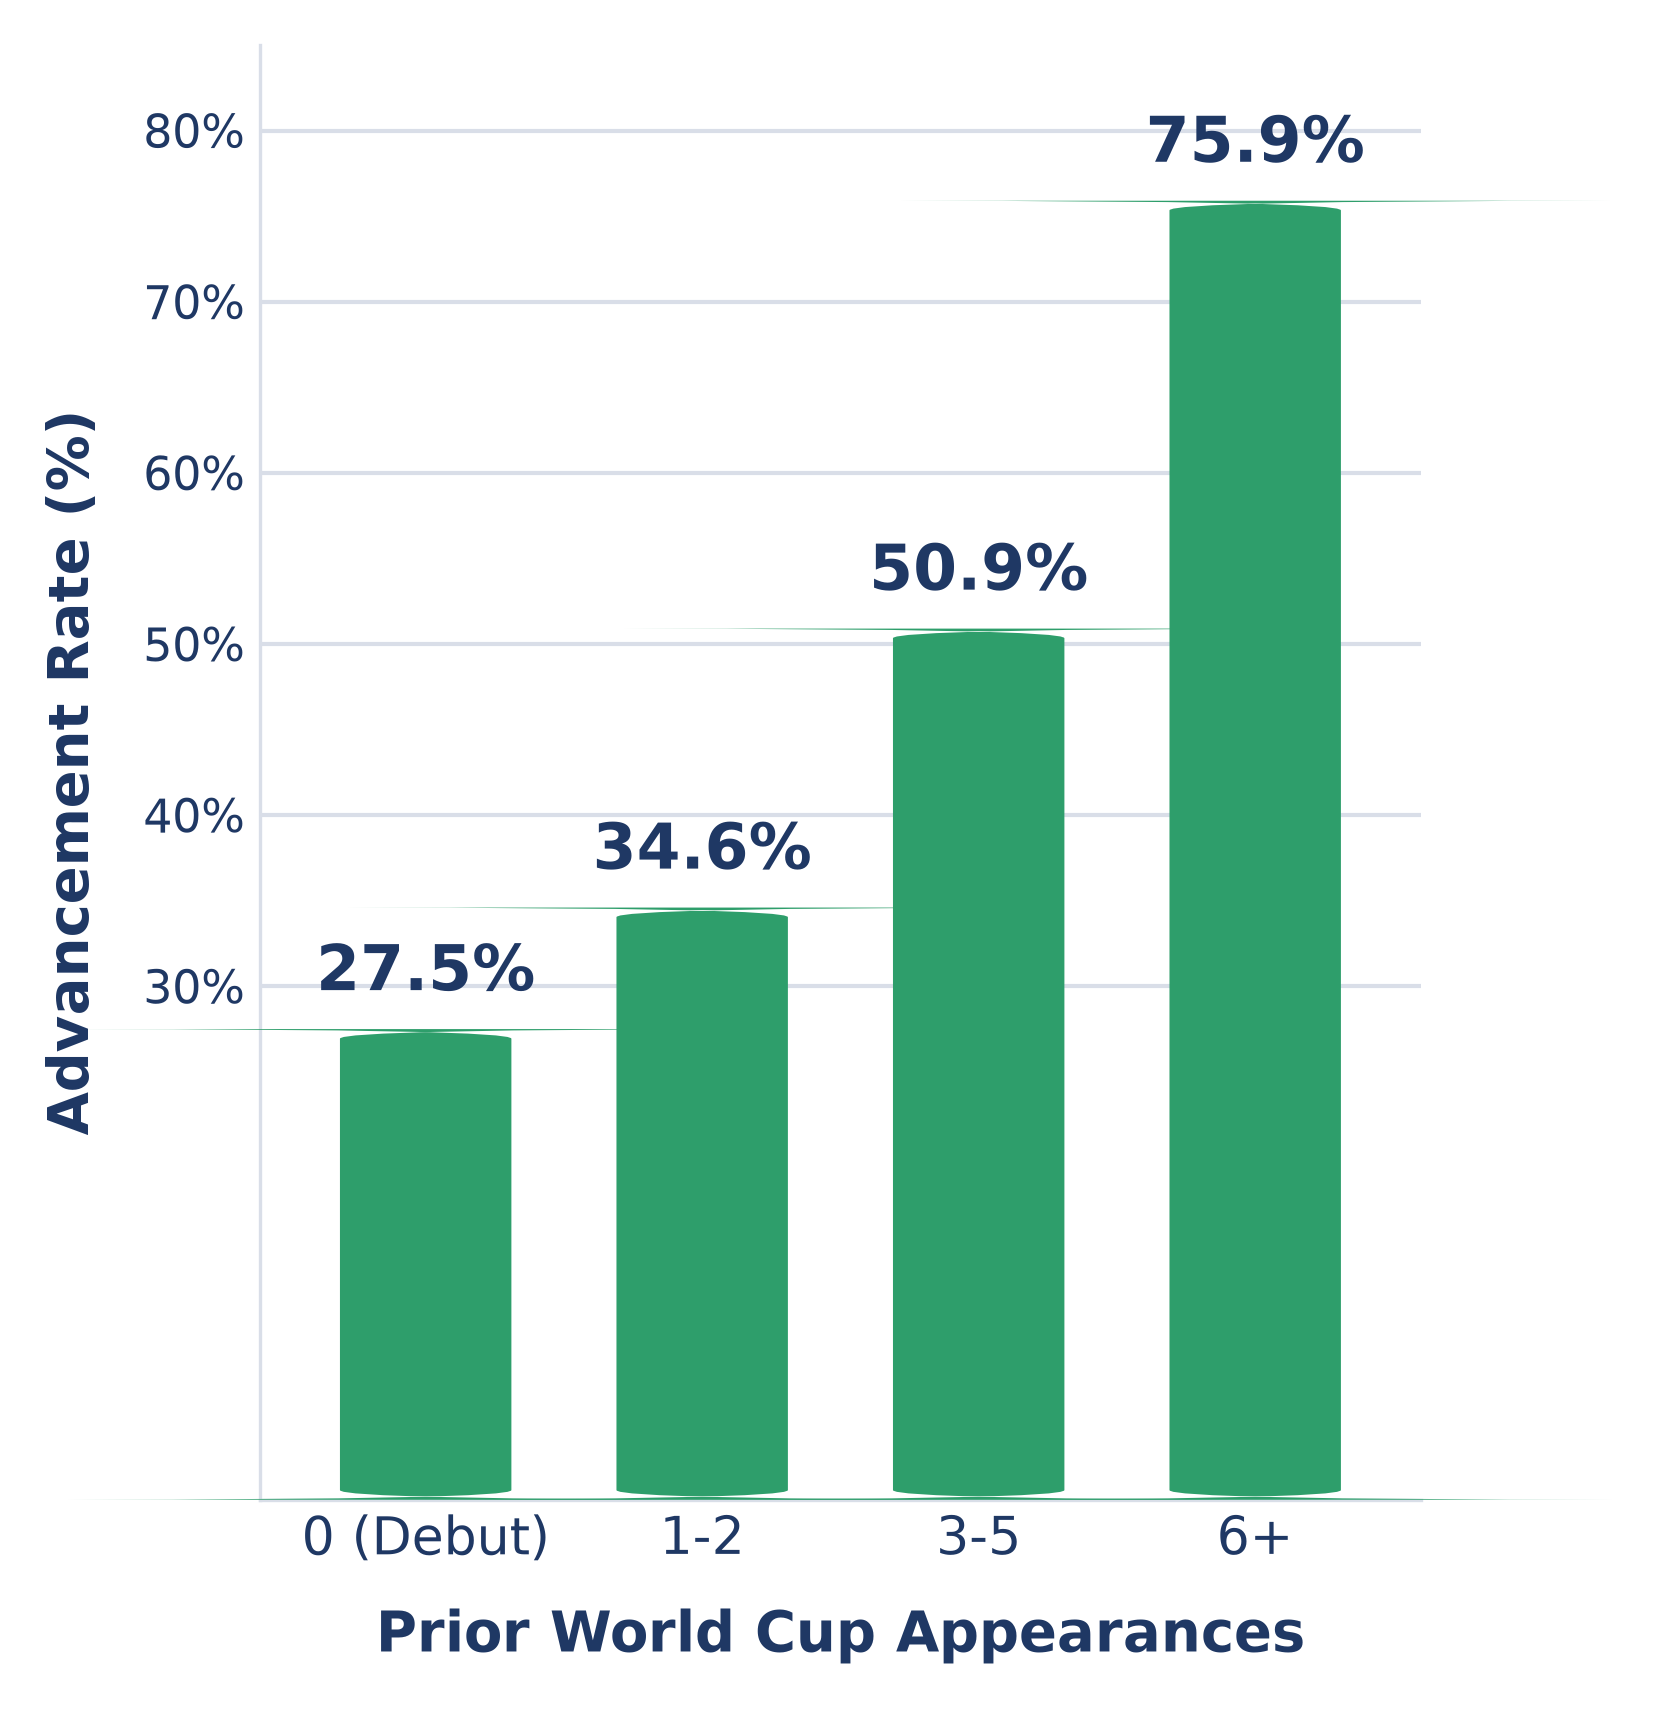
\includegraphics[width=0.75\linewidth]{World_cup_appearances}
    \caption{EDA: probability of advancing rises with number of national World Cup appearances; advancement rates climb from about 28\% for debut teams to about 76\% for teams with six or more prior appearances.}
    \label{fig:eda-exp}
\end{figure}
\vspace*{\fill}
\clearpage

\vspace*{\fill}
\begin{figure}[H]
    \centering
    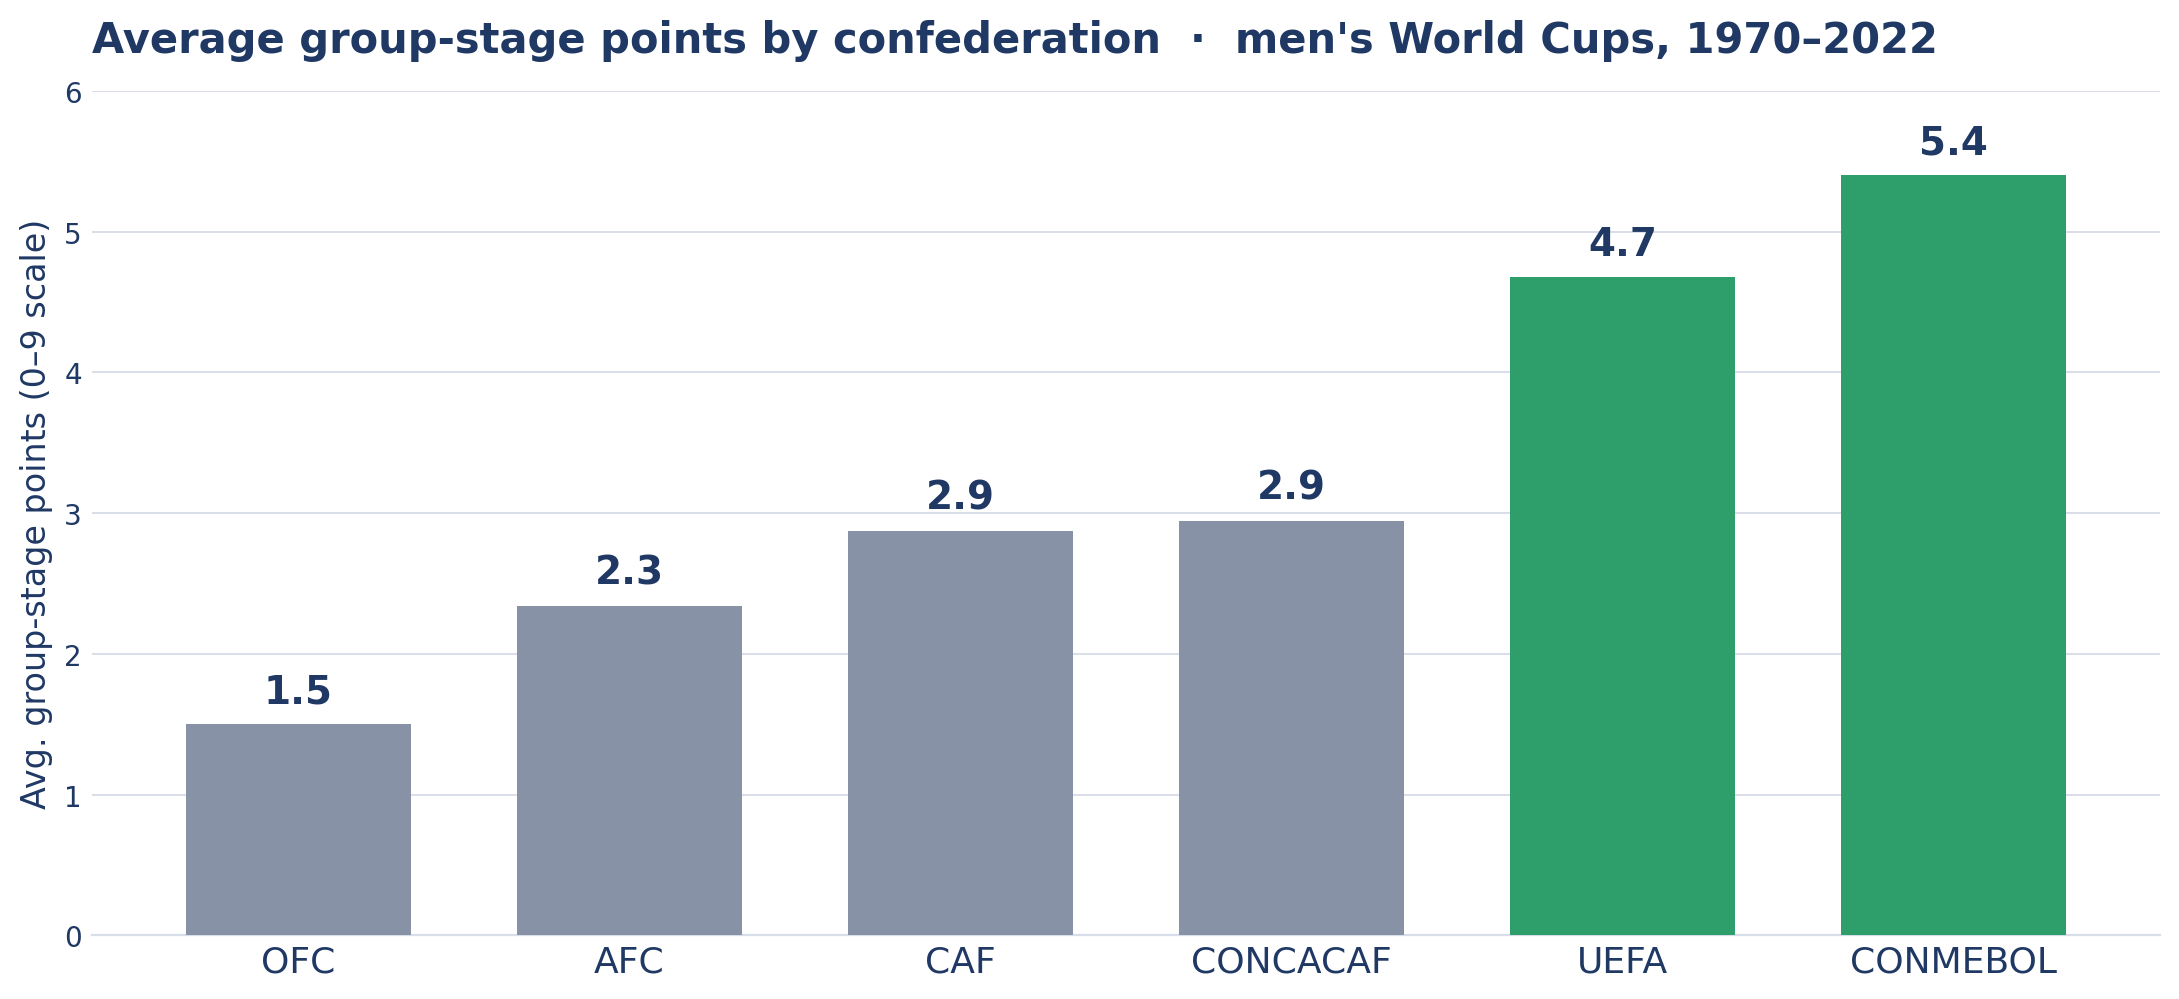
\includegraphics[width=0.8\linewidth]{Group Stage Points per Confederation (deck palette)}
    \caption{EDA: average standardized group-stage points by confederation, men's World Cups 1970--2022. CONMEBOL (5.4) and UEFA (4.7) lead; AFC, CAF, and CONCACAF trail.}
    \label{fig:eda-conf}
\end{figure}
\vspace*{\fill}
\clearpage

\vspace*{\fill}
\begin{figure}[H]
    \centering
    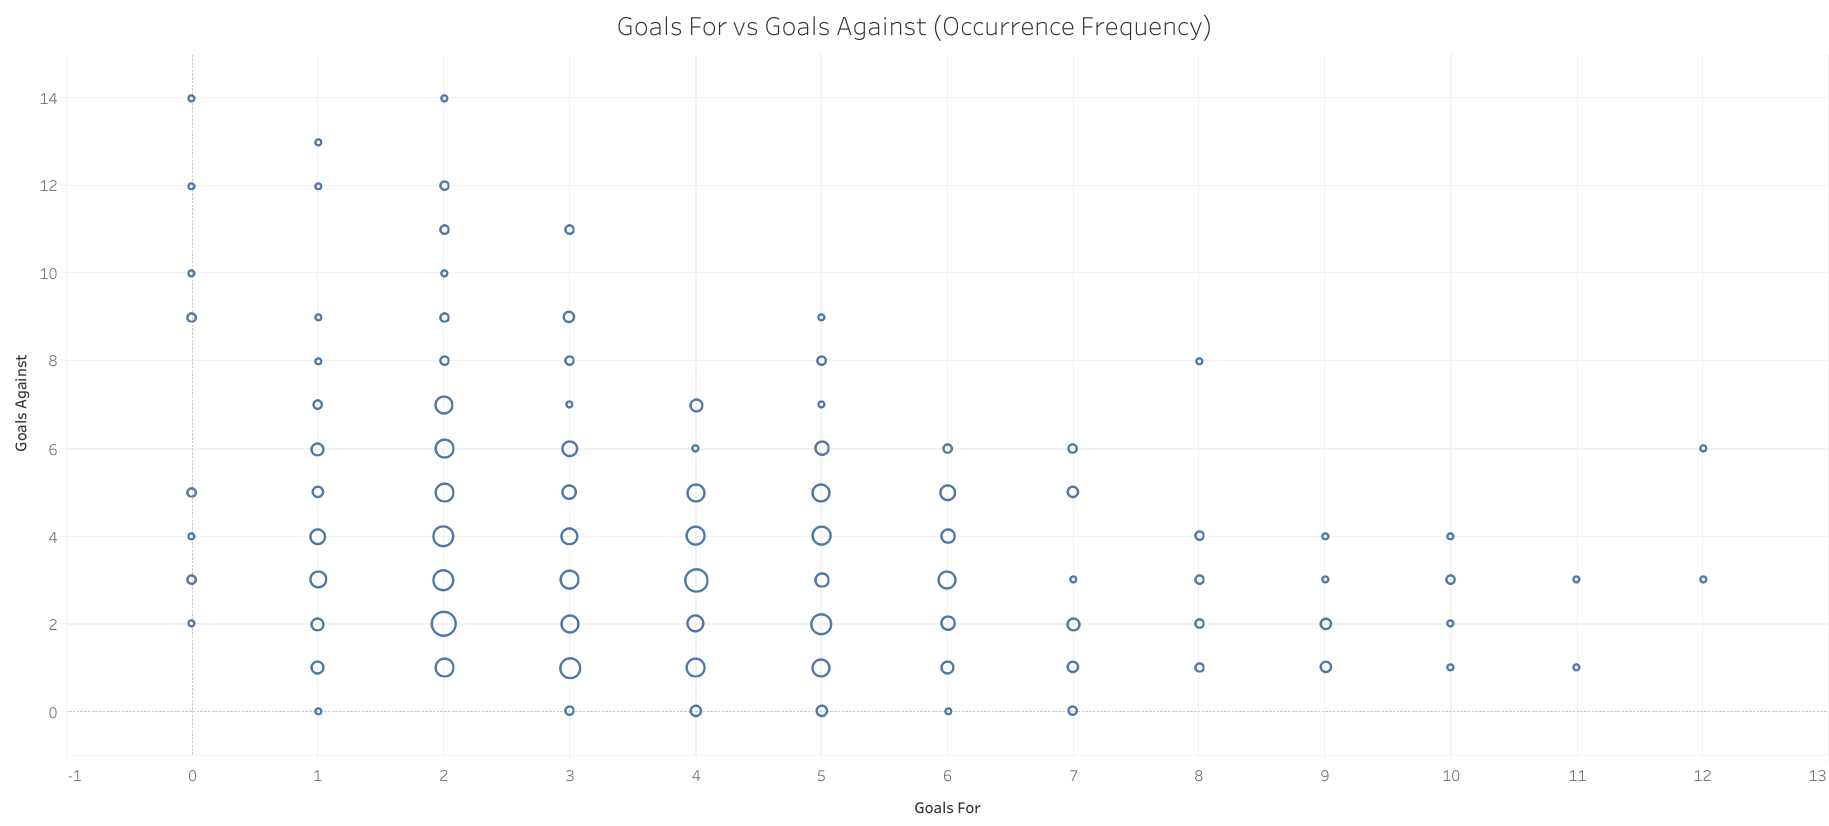
\includegraphics[width=0.75\linewidth]{Goals For vs Goals Against}
    \caption{EDA: count-scaled distribution of goals for versus goals against across the 366 team-campaigns.}
    \label{fig:eda-goals}
\end{figure}
\vspace*{\fill}
\clearpage

% Figure 7. Odds Ratio
\vspace*{\fill}

\begin{center}
    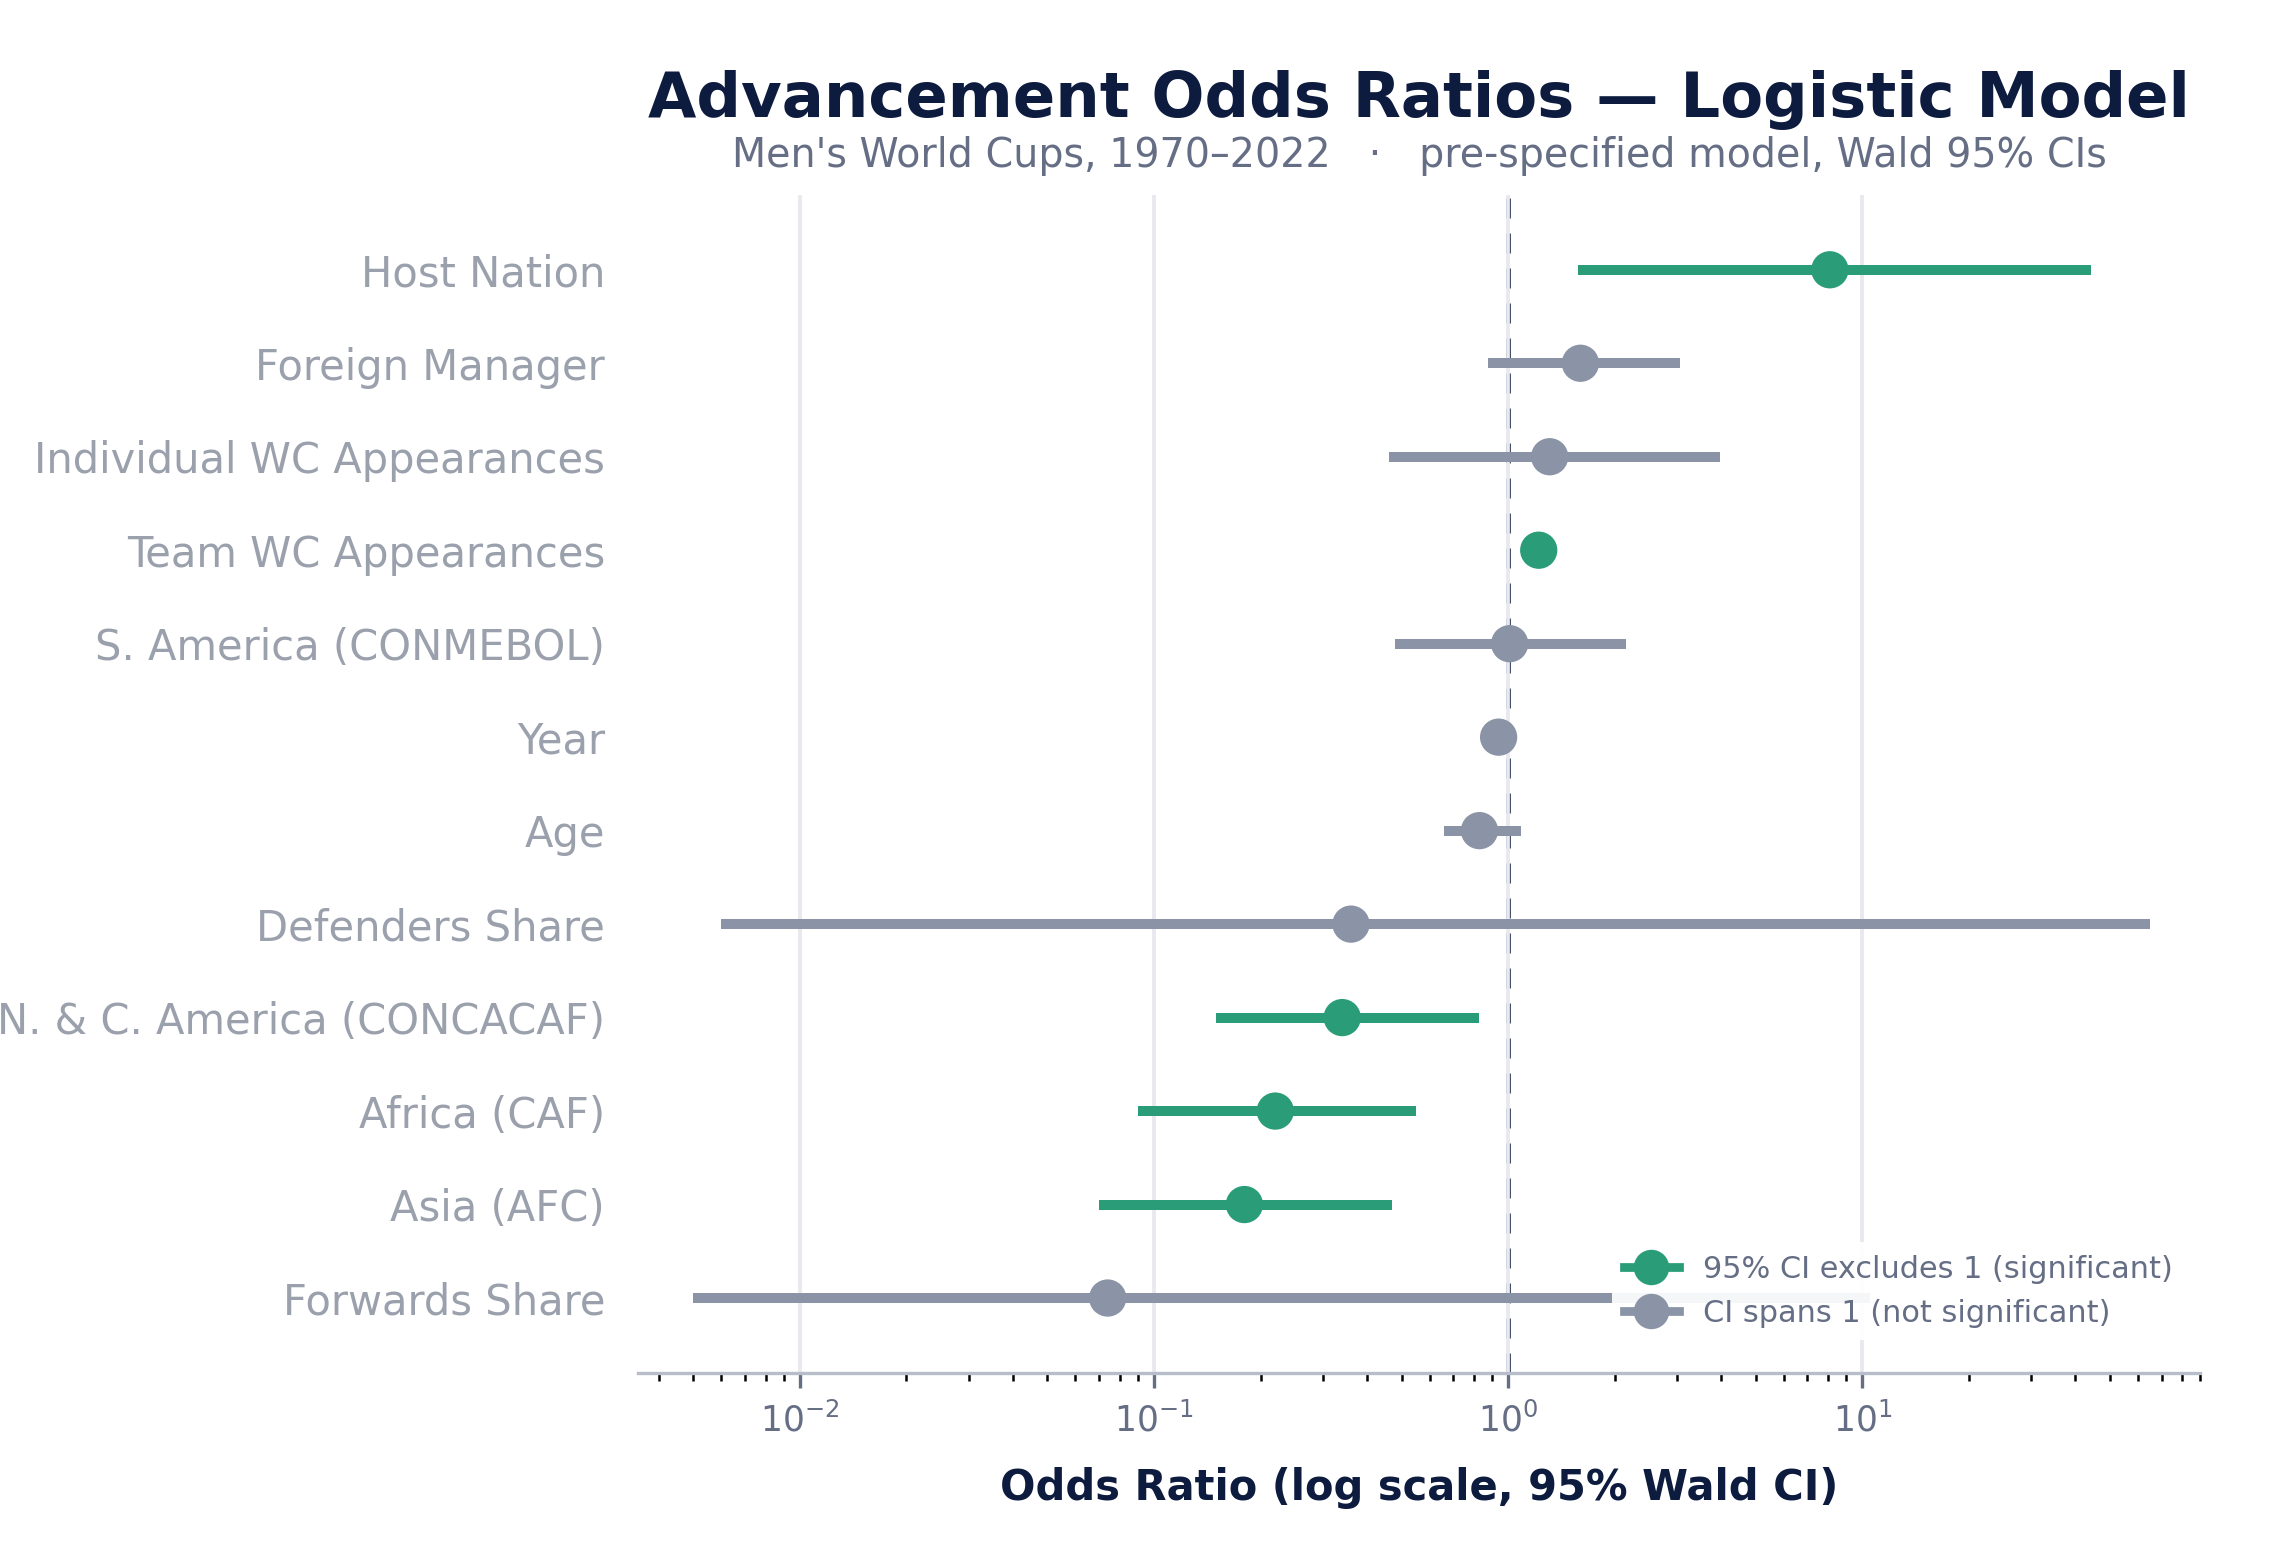
\includegraphics[width=0.7\linewidth]{advancement_odds_ratios_exec.png}
    \vspace{1em}
    \captionof{figure}{Estimated odds ratios (log scale) for advancing beyond the group stage, with 95\% confidence intervals. Host status ($\approx 8\times$) and prior tournaments ($\approx 1.22\times$ per appearance) raise the odds; AFC, CAF, and CONCACAF sit below the UEFA baseline.}
    \label{fig:or}
\end{center}

\vspace*{\fill}
\clearpage

% Figure 8. ROC Curve
\vspace*{\fill}
\begin{figure}[H]
    \centering
    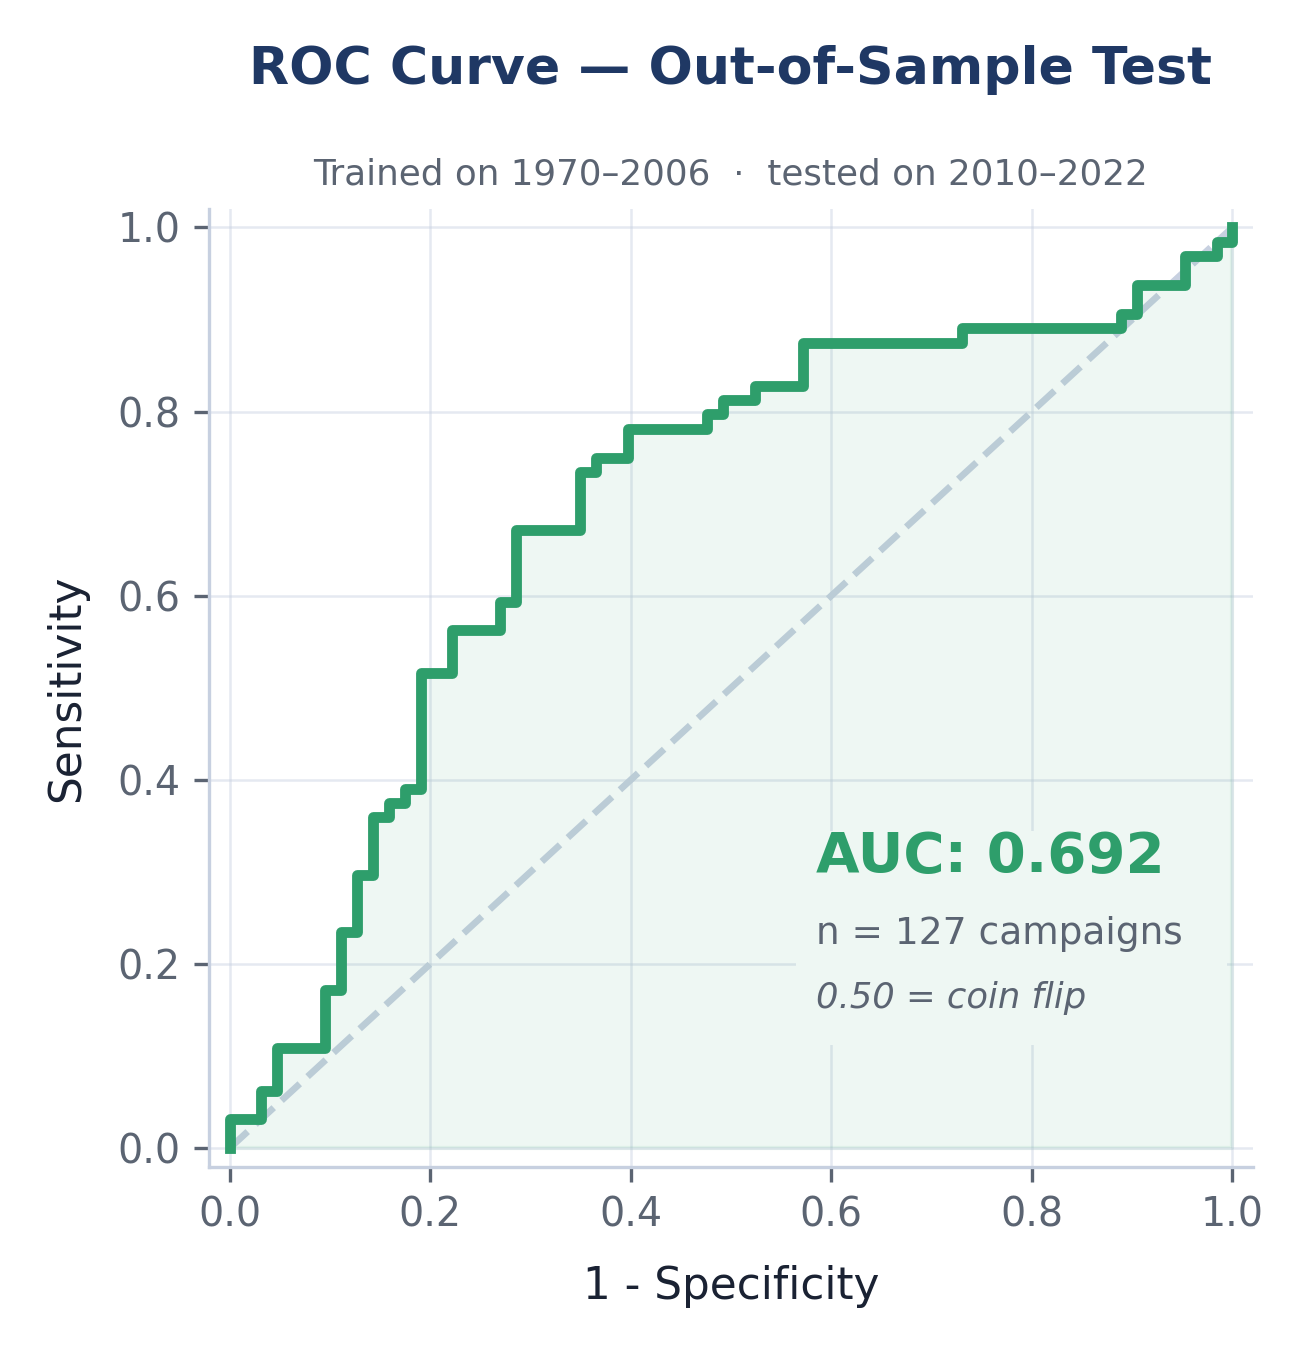
\includegraphics[width=0.55\linewidth]{roc_train_test_split.png}
    \caption{Out-of-sample ROC curve demonstrating predictive performance (AUC = 0.69).}
    \label{fig:roc}
\end{figure}
\vspace*{\fill}
\clearpage

\vspace*{\fill}
\begin{figure}[H]
    \centering
    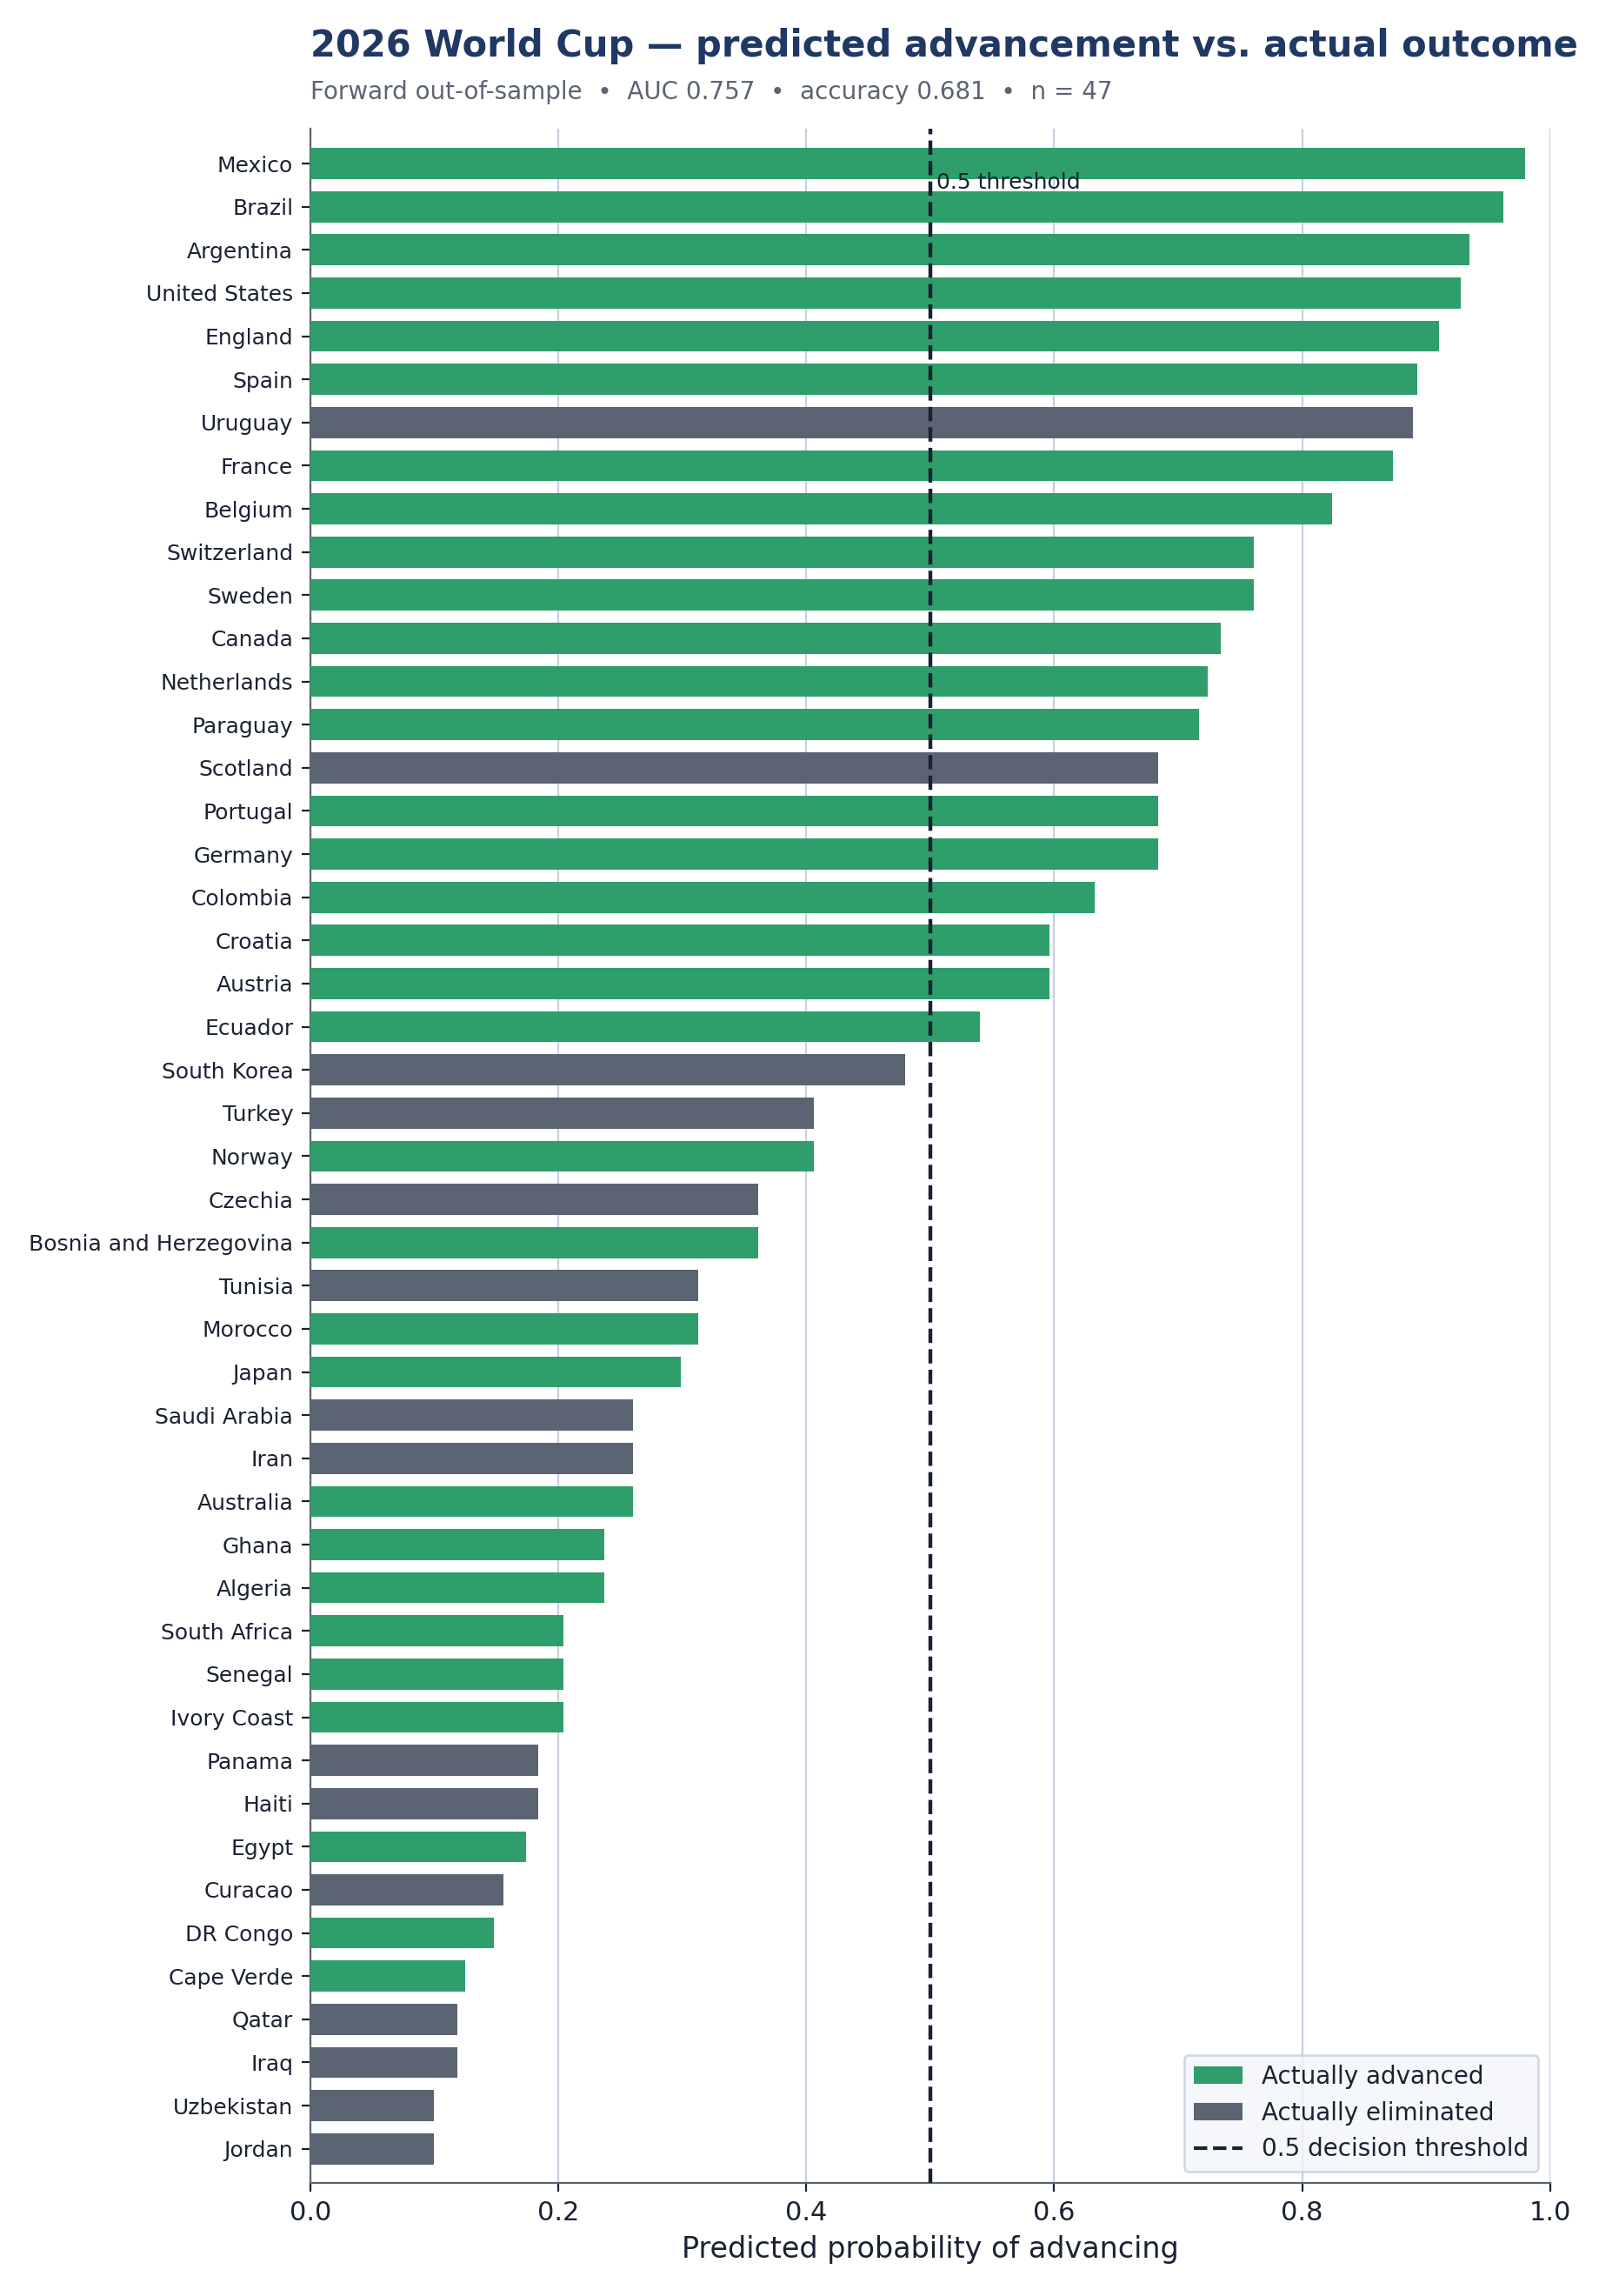
\includegraphics[width=0.6\linewidth]{fig_2026_ranked_probabilities}
    \caption{2026 forward test: all 47 scored teams ranked by predicted probability of advancing, colored by actual outcome, with the 0.5 decision threshold marked (forward-test AUC 0.757, accuracy 0.681).}
    \label{fig:rank2026}
\end{figure}
\vspace*{\fill}
\clearpage

\vspace*{\fill}
\begin{figure}[H]
    \centering
    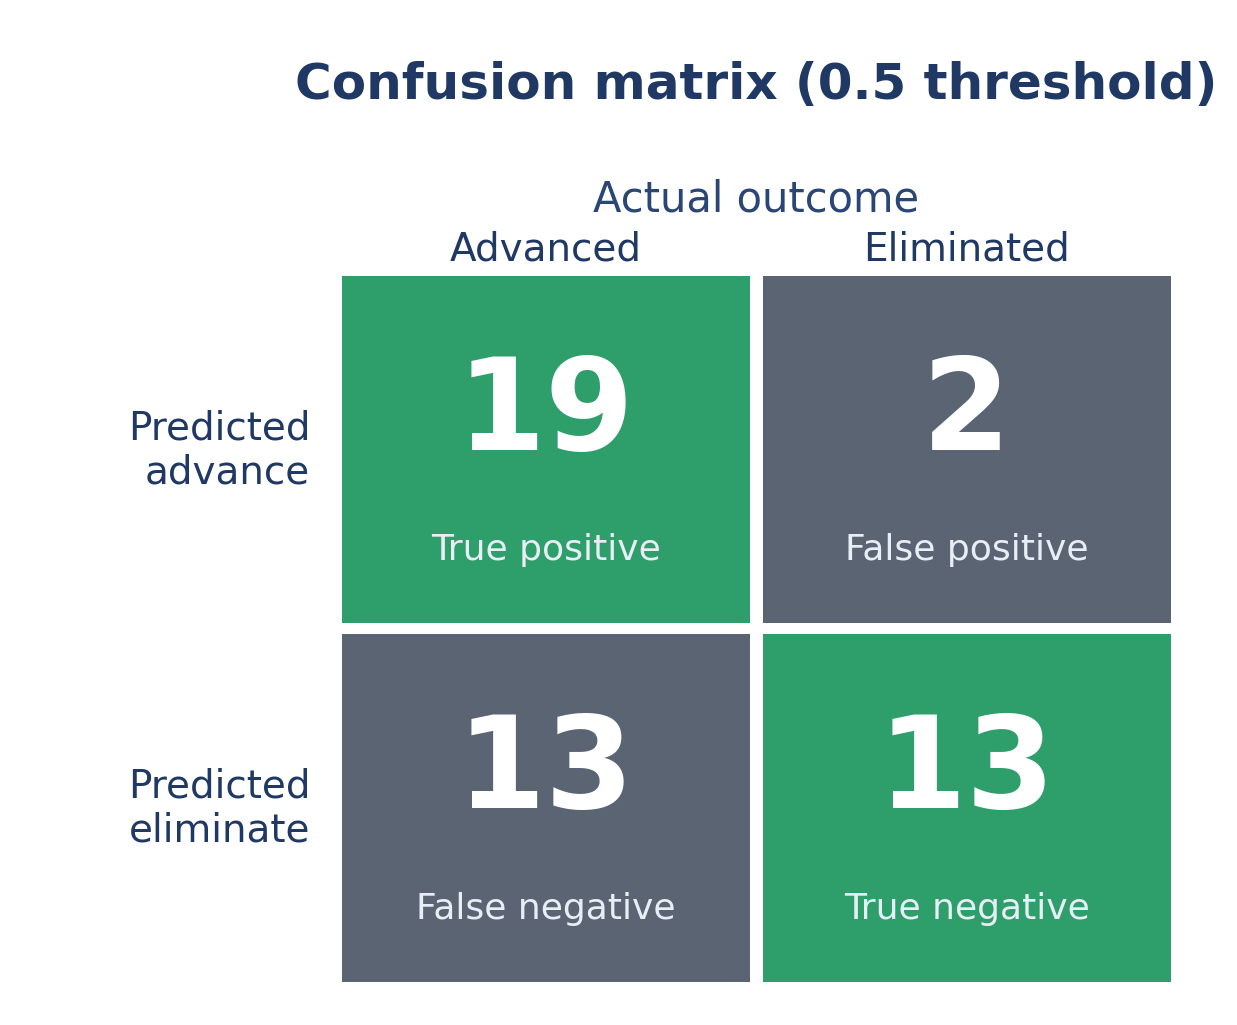
\includegraphics[width=0.6\linewidth]{fig_2026_confusion_matrix}
    \caption{2026 Forward Test: Confusion Matrix at the 0.5 Threshold --- 19 true positives, 13 true negatives, 2 false positives, and 13 false negatives.}
    \label{fig:cm2026}
\end{figure}
\vspace*{\fill}
\clearpage


\section{SQL Queries}
\label{sec:sql}
\lstset{
    language=R,
    basicstyle=\ttfamily\footnotesize,
    keywordstyle=\color{black},
    commentstyle=\color{black},
    stringstyle=\color{black},
    identifierstyle=\color{black},
    numbers=left,
    numberstyle=\tiny,
    stepnumber=1,
    frame=single,
    breaklines=true,
    breakatwhitespace=true,
    columns=fullflexible,
    keepspaces=true,
    showstringspaces=false,
    tabsize=2
}

\vspace{1.2em}
\textbf{Base Dataframe}
\vspace{0.8em}
\begin{lstlisting}
base <- sqldf("
  SELECT gs.tournament_id, gs.team_id, gs.team_name,
         gs.group_name, gs.played, gs.wins, gs.draws, gs.losses,
         gs.goals_for, gs.goals_against, gs.goal_difference,
         gs.points AS points_raw, gs.advanced,
         t.confederation_code, t.region_name,
         tp.year
  FROM group_standings gs
  LEFT JOIN teams       t  ON gs.team_id       = t.team_id
  LEFT JOIN tournaments tp ON gs.tournament_id = tp.tournament_id
  WHERE gs.tournament_name LIKE '%FIFA Men''s%'          -- <- bug fix
    AND gs.stage_name IN ('group stage', 'first group stage')
")


\end{lstlisting}


\vspace{1.2em}
\textbf{Predictor Blocks}
\vspace{0.8em}
\begin{lstlisting}

# --- Team experience: # of prior men's tournaments this team appeared in -----
team_experience <- sqldf("
  SELECT DISTINCT gs.tournament_id, gs.team_id,
    (SELECT COUNT(DISTINCT g2.tournament_id)
       FROM group_standings g2
       JOIN tournaments t2 ON g2.tournament_id = t2.tournament_id
      WHERE g2.team_id = gs.team_id
        AND g2.tournament_name LIKE '%FIFA Men''s%'
        AND t2.year < tp.year) AS prior_tournaments
  FROM group_standings gs
  JOIN tournaments tp ON gs.tournament_id = tp.tournament_id
  WHERE gs.tournament_name LIKE '%FIFA Men''s%'
    AND gs.stage_name IN ('group stage', 'first group stage')
")

# --- Squad composition & age -------------------------------------------------
#     avg_age  = tournament year minus player birth year (approximate).
#       78 players have birth_date = 'not available'; the GLOB guard nulls them
#       so AVG ignores them (otherwise avg_age blows up to ~1400).
#     avg_career_tournaments is LEAKY (whole career incl. future) -> excluded
#       from the model spec; kept here only for reference.
squad_stats <- sqldf("
  SELECT s.tournament_id, s.team_id,
         COUNT(*)                                                           AS squad_size,
         AVG(CASE WHEN substr(p.birth_date, 1, 4) GLOB '[0-9][0-9][0-9][0-9]'
                  THEN tp.year - CAST(substr(p.birth_date, 1, 4) AS INTEGER)
             END)                                                           AS avg_age,
         1.0*SUM(CASE WHEN s.position_code='FW' THEN 1 ELSE 0 END)/COUNT(*) AS forward_share,
         1.0*SUM(CASE WHEN s.position_code='DF' THEN 1 ELSE 0 END)/COUNT(*) AS defender_share,
         AVG(p.count_tournaments)                                           AS avg_career_tournaments
  FROM squads s
  JOIN players     p  ON s.player_id     = p.player_id
  JOIN tournaments tp ON s.tournament_id = tp.tournament_id
  GROUP BY s.tournament_id, s.team_id
")

# --- Squad World Cup experience (CLEAN, non-leaky) ---------------------------
#     Per player, count PRIOR men's World Cups (t2.year < tp.year) then
#     aggregate: avg_prior_wc / max_prior_wc / debutant_share.
squad_experience <- sqldf("
  SELECT s.tournament_id, s.team_id,
         AVG(prior)                                            AS avg_prior_wc,
         MAX(prior)                                            AS max_prior_wc,
         1.0*SUM(CASE WHEN prior=0 THEN 1 ELSE 0 END)/COUNT(*) AS debutant_share
  FROM (
    SELECT s.tournament_id, s.team_id, s.player_id,
      (SELECT COUNT(DISTINCT s2.tournament_id)
         FROM squads s2
         JOIN tournaments t2 ON s2.tournament_id = t2.tournament_id
        WHERE s2.player_id = s.player_id
          AND s2.tournament_name LIKE '%FIFA Men''s%'
          AND t2.year < tp.year) AS prior
    FROM squads s
    JOIN tournaments tp ON s.tournament_id = tp.tournament_id
    WHERE s.tournament_name LIKE '%FIFA Men''s%'
  ) s
  GROUP BY s.tournament_id, s.team_id
")

# --- Group-stage discipline (cards). Recorded from 1970 on. ------------------
cards <- sqldf("
  SELECT tournament_id, team_id,
         SUM(yellow_card)                     AS yellows,
         SUM(red_card + second_yellow_card)   AS reds,
         COUNT(*)                             AS total_cards
  FROM bookings
  WHERE stage_name = 'group stage'
  GROUP BY tournament_id, team_id
")

# --- Host nation flag --------------------------------------------------------
host <- sqldf("SELECT DISTINCT tournament_id, team_id, 1 AS is_host
               FROM host_countries")

# --- Foreign manager flag (approx: manager country != team name) -------------
manager <- sqldf("
  SELECT tournament_id, team_id,
         MAX(CASE WHEN country_name <> team_name THEN 1 ELSE 0 END) AS foreign_manager
  FROM manager_appointments
  GROUP BY tournament_id, team_id
")
\end{lstlisting}
\clearpage


\textbf{Assemble Model Query}
\vspace{0.8em}
\begin{lstlisting}
model_full <- sqldf("
  SELECT b.*,
         e.prior_tournaments,
         sq.squad_size, sq.avg_age, sq.forward_share, sq.defender_share,
         sq.avg_career_tournaments,
         xp.avg_prior_wc, xp.max_prior_wc, xp.debutant_share,
         COALESCE(c.yellows, 0)         AS yellows,
         COALESCE(c.reds, 0)            AS reds,
         COALESCE(c.total_cards, 0)     AS total_cards,
         COALESCE(h.is_host, 0)         AS is_host,
         COALESCE(m.foreign_manager, 0) AS foreign_manager
  FROM base b
  LEFT JOIN team_experience  e  
        ON b.tournament_id=e.tournament_id  AND b.team_id=e.team_id
  LEFT JOIN squad_stats      sq  
        ON b.tournament_id=sq.tournament_id AND b.team_id=sq.team_id
  LEFT JOIN squad_experience xp 
        ON b.tournament_id=xp.tournament_id AND b.team_id=xp.team_id
  LEFT JOIN cards            c  
        ON b.tournament_id=c.tournament_id  AND b.team_id=c.team_id
  LEFT JOIN host             h  
        ON b.tournament_id=h.tournament_id  AND b.team_id=h.team_id
  LEFT JOIN manager          m  
        ON b.tournament_id=m.tournament_id  AND b.team_id=m.team_id
")
\end{lstlisting}


\clearpage
\section{References}

\textbf{Schauberger, G., \& Groll, A. (2018)}. Predicting matches in international football tournaments with random forests. \emph{Statistical Modeling}. \url{https://doi.org/10.1177/1471082X18799934}

\noindent \textbf{Szczecinski, L., \& Roatis, I. I. (2022)}. FIFA ranking: Evaluation and path forward. \emph{Journal of Sports Analytics}. \url{https://doi.org/10.3233/JSA-200619}

\noindent \textbf{Fjelstul, J. C. (2023)}. The Fjelstul World Cup Database (Version 1.2.0) [Data set]. GitHub. \url{https://github.com/jfjelstul/worldcup}

\noindent \textbf{The Global Statistics. (2026, July 20)}. FIFA World Cup 2026 revenue statistics: Key facts. \url{https://www.theglobalstatistics.com/fifa-world-cup-revenue-statistics/}

\end{document}

